\documentclass[conference]{IEEEtran}
\IEEEoverridecommandlockouts
% The preceding line is only needed to identify funding in the first footnote. If that is unneeded, please comment it out.
\usepackage{cite}
\usepackage{amsmath,amssymb,amsfonts}
\usepackage{algorithmic}
\usepackage{graphicx}
\usepackage{empheq}
\usepackage{textcomp}
\usepackage{xcolor}
\usepackage{fancyhdr}
\usepackage[utf8]{inputenc}
\def\BibTeX{{\rm B\kern-.05em{\sc i\kern-.025em b}\kern-.08em
    T\kern-.1667em\lower.7ex\hbox{E}\kern-.125emX}}
    


\begin{document}

\title{Model Predictive Control for \\Adaptive Cruise Control}

\author{
\IEEEauthorblockN{Nikhil Nagendra (5049628),\\n.hudralinagendra@student.tudelft.nl}

\and
\IEEEauthorblockN{Yen-Lin Wu (4848489),\\Y.Wu-29@student.tudelft.nl}

}

\maketitle
\thispagestyle{fancy}

\begin{abstract}
A model predictive control (MPC) approach is implemented on Adaptive Cruise Control system. 
\end{abstract}

\begin{IEEEkeywords}
 ACC, MPC
\end{IEEEkeywords}

\section{Introduction}
\subsection{Adaptive Cruise Control in literature}

Adaptive cruise control (ACC) is an enhancement of the conventional cruise control which is currently standardised in most modern commercialised vehicles. The purpose of a classical cruise control is to maintain longitudinal vehicle velocity by tracking the velocity as requested by the driver. In ACC, there is an additional tracking of the velocity of the vehicle ahead and adapting to it, by accelerating or braking the vehicle independently of the driver. Typically, an external sensor such as a radar is used to detect the vehicle ahead and measure relative velocity between the vehicles \cite{Elsevier}.
ACC systems consist of two subsystems: a vehicle dependent part and a vehicle independent part. The former calculates a required acceleration/deceleration profile for the vehicle. The controller part forms the dependent part which tracks the profile by actuating the throttle and brake system \cite{Moon}. A schematic of the ACC system is shown in Fig. \ref{fig:Schematic_ACC}. 

\begin{figure}[h]
\centering
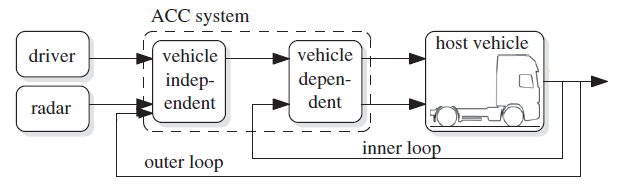
\includegraphics[width=0.45\textwidth]{img/ACC_schematic.png}\\
\caption{Schematic of ACC system \cite{Elsevier}}
\label{fig:Schematic_ACC}
\end{figure}
% Revisit schematic to also include the variables present in the figure

The main control objective is to follow the vehicle ahead. However, there are other aspects also considered such as comfort, fuel economy and safety \cite{Elsevier}. It should be noted that ACC is more of a comfort system than a safety system as the deceleration is limited to 3 $m/s^2$. Also, function of stop-and-go system can be integrated with ACC in order to allow the vehicle to stop behind vehicles at traffic signals or other conditions and continue again when the vehicle ahead begins to move \cite{ACC_SG}.  Also, driver mental workload was reduced with the implementation of ACC. Since ACC takes control from the driver, it should resemble the driver’s behaviour to a certain extent. Furthermore, constraints from subjective specific desirable behaviour should also be considered. Because of the need for constraints, classical controllers such as PID controller are insufficient. With LQR controller, it was found that the response of the system was slower compared with Model Predictive Controller (MPC) \cite{Takahama}. There are 2 approaches to design controllers for linear systems with constraints: anti-windup control and MPC. Former one demonstrates adequate performance on Single-Input Single-Output (SISO) situations, whereas MPC has outperformed in the field of complex constrained multi-variable (Multi-Input Multi-Output or MIMO) control problems. Other main advantages of MPC here would be the on-line optimisation of the system, stability and feasibility guarantee with closed loop MPC, and implementation in a receding horizon manner, where the optimization problem is solved in every time step. This enables the controller to adapt to actual working conditions, i.e. traffic situations, and, as such, the controller is situation dependent. The advantage of MPC for ACC is that high control performance can be obtained since constraints such as small feedback gain for LQR controller can be exclusively dealt with and the tuned weighing parameters can be intuitively and flexibly considered as a function of time considering various driving situations \cite{Takahama}.


% Also include the explanation of different sections of the paper.
\subsection{Model}

The host vehicle and target vehicle are modelled as in Fig. \ref{fig:ACC_example} with a relative distance.

\begin{figure}[h]
\centering
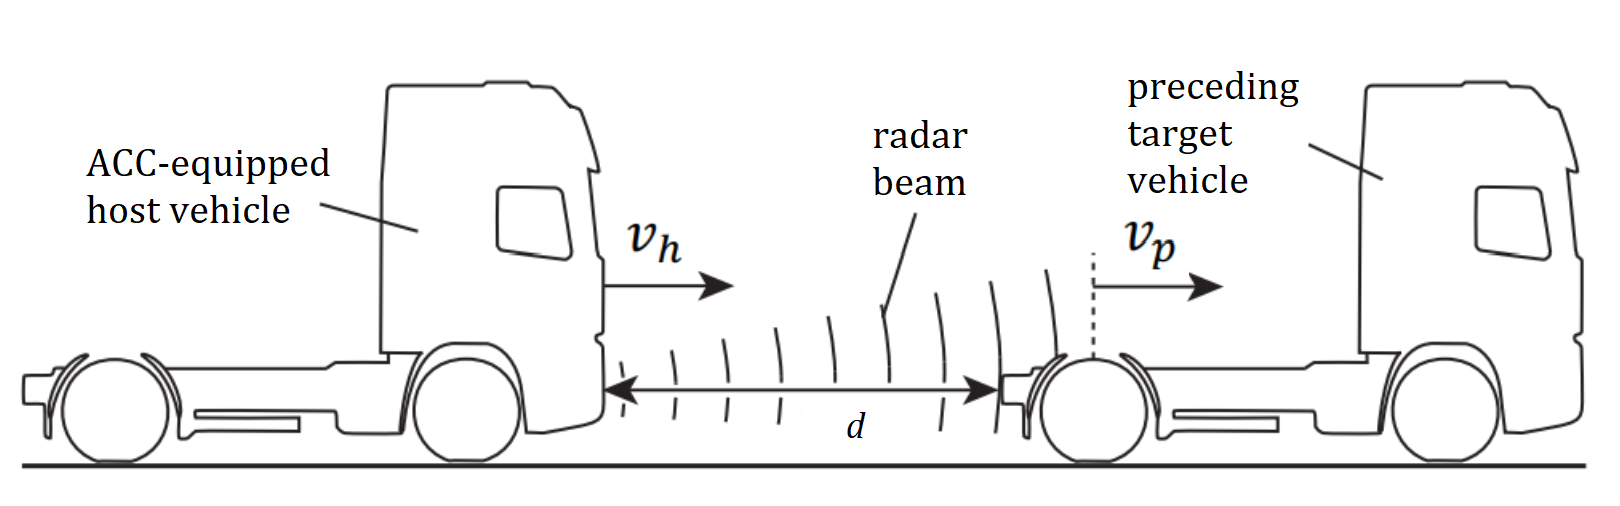
\includegraphics[width=0.45\textwidth]{img/trucks.png}\\
\caption{Example of ACC working principle. The host vehicle, driving with velocity $v_h$ and acceleration $a_h$, is equipped with ACC, which measures the preceding target vehicle, with velocity $v_t$. A radar measures the distance $x_r$ and the relative velocity $v_r=v_t-v_h$ between the vehicles. \cite{Elsevier}}
\label{fig:ACC_example}
\end{figure}

Since the purpose of ACC is to maintain a desired distance between host and target vehicle, a problem of the below considerations is taken,
\begin{itemize}
    \item The distance error $\delta d$, defined as difference between the inter-vehicle distance $d$ and desired distance $d_r$, where $\delta d = d - d_r$. This error should converge to zero.
    \item The velocity error $\delta v$, defined as the difference between the preceding target vehicle velocity $v_p$ and host velocity $v_h$. This error also should converge to zero.
    \item Acceleration of the host vehicle $\dot{v}_h$, which should also converge to zero.
\end{itemize}

A vehicle dynamics model is also considered to design MPC and analyse the controller performance. The longitudinal dynamics of the host vehicle is given as,
\[m\dot{v}_h = ma_f - r_{travel}\]
Here, m is the mass of the vehicle, $v_h$ the host vehicle velocity, $a_f$ is the traction force of the host vehicle converted to acceleration and $r_{travel}$ is the travel resistance consisting of several factors.
In general, the actuation dynamics can be described as an ordinary differential equation as below,
\begin{gather}
\begin{aligned}
\dot{x}_f &= f_{act}(x_f,u)\\
a_f &= h_{act}(x_f)
\end{aligned}
\end{gather}

where $x_f \in \mathbb{R} ^{n_f}$, $u \in \mathbb{R}$ are the states and the input to actuation system respectively. \textit{u} is the acceleration command calculated by the ACC controller. The output of the system is y = $a_f$. It is to be noted that since we are taking a simple model, we neglect the travel resistance $r_{travel}$ as it contains several factors which are vehicle specific. 

For the plant model of the ACC system, two primary state variables are taken, $\delta d$ and $\delta v$ as described earlier. The variable $d_r$ defined in $\delta d$ is given based on the constant time headway given as
\[d_r = T_{hw}v_h + d_0\]
where $T_{hw}$ is the constant time headway (the time needed for the host vehicle to reach the current position of the target vehicle) and $d_0$ is the stopping distance for safety margin. Here, we do not consider the stop-and-go function where the vehicle stops completely if the target vehicle stops. Hence we take $d_0$ as zero.

Now we define the state variable of the plant as,
\begin{align*}
    x = \begin{bmatrix}
    x_1 & x_2 & x_3^T
    \end{bmatrix}
\end{align*}
with $x_1 = \delta d$, $x_2 = \delta v$ and $x_3 = x_f$.\\
The state-space model can now be formulated as,
\begin{gather}
\begin{aligned}
\dot{x}_f &= A_f(t)x_f + B_f(t)u\\
a_f &= C_f x_f
\end{aligned}
\end{gather}

where the state $x_f \in \mathbb{R}$, i.e. $n_f=1$ and

\begin{equation}
A_f(t) =
\begin{cases}
& -\frac{1}{T_{eng}},\: \text{if}\: u(t) \geq a_{thr\_off}\\
& -\frac{1}{T_{brk}},\: \text{if}\: u(t) < a_{thr\_off}
\end{cases}
\end{equation}

\begin{equation}
B_f(t) =
\begin{cases}
& -\frac{K_{eng}(t)}{T_{eng}},\: \text{if}\: u(t) \geq a_{thr\_off}\\
& -\frac{K_{brk}(t)}{T_{brk}},\: \text{if}\: u(t) < a_{thr\_off}
\end{cases}
\end{equation}

\[
C_f = 1
    % \begin{bmatrix}
    % 1 & 0 & 0\\
    % 0 & 1 & 0\\
    % 0 & 0 & 1
    % \end{bmatrix}
\]

$T_{eng}$ and $T_{brk}$ are given respectively as the time constant of acceleration using engine and deceleration using brake, $a_{thr.off}$ is the acceleration generated when the throttle valve is closed, $K_{eng}(t)$ and $K_{brk}(t)$ are the steady-state gains dependent on time. In the system (1), the dynamics is separated into acceleration and deceleration side and simply modeled as first-order delay system. Therefore, the overall simplified linear state-space model with the three states can be written as,
\begin{gather}
\begin{aligned}
\dot{x} &= A(t)x + B(t)u\\
y &= Cx
\end{aligned}
\end{gather}

where $x \in \mathbb{R}^3$ and

\[
A(t)=
    \begin{bmatrix}
    0 & 1 & -T_{hw}\\
    0 & 0 & -1\\
    0 & 0 & A_f(t)
    \end{bmatrix},
    \quad
B(t)=
\begin{bmatrix}
0\\
0\\
B_f(t)
\end{bmatrix}
\]

This model will be used for our MPC problem. For a non-linear system, it is necessary to linearize the system around the equilibrium. However, since we have already considered a linear system, we directly discretize the system from continuous time to discrete time. In MATLAB, this is done using the \textit{c2d} command. By doing so, we get the below discretized model.
\begin{gather}
\begin{aligned}
    x_{t+1} &= \Pi(t) x_t + \Gamma(t) u_t\\
    y_t &= C_d x_t
\end{aligned}
\end{gather}

$\Pi(t) = (I+T_S A(t)),\, \Gamma(t)=T_S B(t)$ and $C_d=C$ where $T_S$ is the sampling time.

% from MATLAB we need to write the values and rewrite the above equation.
    



\section{Model Predictive Control Design}
In this section, a model predictive control method is designed to maintain a constant distance between the target and host vehicle. Different MPC design methods were considered. 
\begin{itemize}
    \item Regulation of system using state-based MPC.
    \item Output MPC with reference tracking.
\end{itemize}
To solve the MPC problem at every iteration, we define a general cost function as given in %REF the textbook
. This cost function is defined as follows,
\begin{equation}
   V_N(x_0,u) &= \sum_{k=0}^{N-1}\big\{l(x(k),u(k)\}+V_f\big(x(N)\big)\\
   \label{Cost function}
\end{equation}
\begin{center}
    s.t. $u\in \mathbb{U}, x \in \mathbb{X}$
\end{center}

\subsection{Regulation MPC}
Here, the distance error $\delta d$, the velocity error $\delta v$ and acceleration $\dot{v}_h$ has to be controlled to converge to the origin for a given control input command, i.e, acceleration.
The states considered have to be constrained in order to meet the required distance and velocity between the vehicles. The ACC system is a comfort system and hence the accelerations are limited to $\dot{v}_{h_{min}}$ = $u_{min} = -3.0 m/s^2$. The maximum acceleration however depends on the $v_p$. Due to the different nature of engines between the vehicles, it may not be possible to achieve the same acceleration. Hence, the maximum acceleration $\a_{h_{max}}$ is bounded. The relation between $\dot{v}_h$ and $v_p$ is chosen linear due to the MPC problem taken. Therefore, $u_{h_{max}} = 3(1 - 0.025\cdot v_h) m/s$ \cite{ACC_SG}. It is assumed that the $v_h=40 m/s$ which results in $u_{h_{max}} = 0$. Also, a constraint is added on the rate of change of acceleration $\dot{u}$ in order to minimise jerks. This constraint is set to $|\delta \dot{u}| = 5 m/s^3$.
Finally a minimum relative distance has to be set. The relative distance has to be larger than the minimum relative distance in order to avoid collision with the preceding target vehicle.
Therefore the control constraints are defined as,
% Inequalities for constraints
State boundaries are defined as follows,
\begin{itemize}
    \item Maximum and minimum $v_h$: Here, only longitudinal movement of the host vehicle is considered.
    \item Maximum and minimum $v_p$: Here, only longitudinal movement of the preceding target vehicle is considered as well. Also, it is assumed that the maximum $v_h$ is the same as the $v_p$ and both are moving in the same direction.
    \item Since we do not consider stop-and-go function, we put limits on $v_p$ as $15 < v_t \leq v_{t_{max}}$.
    \item Maximum relative distance is the maximum range of the radar. % REVISIT
\end{itemize}

\begin{equation}
\label{condition1}
    m=
    \begin{bmatrix}
    0 \\ 0 \\ -3
    \end{bmatrix}
    \leq
    \begin{bmatrix}
    \delta d \\ \delta v \\ u \\
    \end{bmatrix}
    \leq
    \begin{bmatrix}
    2 \\ 2.5 \\ 5 \\
    \end{bmatrix}
    =M
\end{equation}
The MPC optimisation problem to be solved for each iteration is represented by the equation ({\ref{Cost function}}) and hence is given as,
\begin{gather}
    \begin{aligned}
        l\big(x(k),u(k)\big) &= x(k)^TQx(k) + u(k)^TRu(k)\\
        V_f\big(x(N)\big) &= x(N)^TPx(N)
    \end{aligned}
\end{gather}
where Q = ... , R = ... and P is the solution of the Discrete Algebraic Riccati Equation (DARE). P,Q and R are positive definite in this case. The values of R and Q were obtained in an iterative manner. 

\subsection{Output MPC}
To simulate output-based control as is the case in ACC, an output MPC controller was designed. Here, we assume there are no disturbances (they will be present, however for simplicity we will neglect it in this case). First we need to check whether the system is observable and controllable in order to design an observer state model. For reference tracking, an optimal target selection (OTS) needs to be solved offline in order to obtain $x_{ref}$ and $u_{ref}$. The OTS problem is then given as below,

% Slide 6 from mpc_lec5 equations
\begin{equation}
(x_{ref}, u_{ref})(y_{ref}) \in
\begin{cases}
& \underset{x_r, u_r}{\arg\max} \: J(x_r, u_r)\\
& \text{s.t.} \begin{bmatrix}
                    I-A & -B \\
                    C & 0
                \end{bmatrix}
                \begin{bmatrix}
                x_r \\ u_r
                \end{bmatrix}
                =
                \begin{bmatrix}
                0 \\ y_{ref}
                \end{bmatrix}\\
& \quad\quad\quad  (x_r, u_r) \in \mathbb{Z} \\
& \quad\quad\quad Cx \in \mathbb{Y}
\end{cases}
\end{equation}

For the observer, the Kalman gain L is obtained with the weighing matrices Q - diag() and R = .. It is verified that with the new A matrix given by ($\Pi$ - LC), the error dynamics is asymptotically stable. 


\section{Asymptotic Stability}
In this section, we show that the MPC controller strategy proposed in section \cite{textbook} %REF to Section I 
asymptotically stabilizes the closed loop system given that the system initial conditions are sufficiently close to the origin. 

We need to verify the following 2 auxiliary results:\\
1) $\mathbb{X} _f \subseteq \{x \in \mathbb{X} \mid Kx \in \mathbb{U} \}$\\
2) $x \in \mathbb{X}_f \Rightarrow A_K x \in \mathbb{X} _f$

To prove 1), we suppose $x \in \mathbb{X}_f$ holds. We have $x^T Px \leq 5$. Note that $\mathbb{X}=\{x \in \mathbb{R} ^3 | m \leq x \leq M \}$, as proposed in equation (\ref{condition1}), describes a 3-dimensional constraint.

% lec4 p.7,8
Asymptotic (Exponential) Stability:
$l(x,u) = \frac{1}{2}(x^T Qx + u^T Ru) \geq \frac{1}{2}x^T Qx \geq \frac{1}{2} \lambda_{min}(Q)|x|^2$
$V_f (x) = \frac{1}{2}x^T Px \leq \frac{1}{2}\lambda_{max}(P)|x|^2$

\section{Numerical Simulation}
In the simulation, the controller sampling time $T_s$ is 0.05 sec. The constant time headway $T_{hw}$ is 1.3 sec. The prediction horizon $p=20$ and control horizon $c=1$ are chosen to be as small as possible. 


\begin{table}[h]
\begin{center}
\caption{The parameters of the actuation system model}
\begin{tabular}{| c | c | c | c |} %\toprule[1.5pt]
%\caption{Vehicle parameters}
\hline
T_{eng} & 0.460 \\
\hline
K_{eng} & 0.732 \\
\hline
T_{brk} & 0.193 \\
\hline
K_{brk} & 0.979 \\
\hline
\end{tabular}
\label{Tab parameters}

\end{center}
\end{table}


\section{Conclusions}
One of the drawbacks of MPC lies in its calculation loads that is derived from the optimisation problems considering future prediction in every sampling period.


\bibliographystyle{unsrt}
\bibliography{bibliography}

\end{document}
